% GNUPLOT: LaTeX picture with Postscript
\begingroup
  \makeatletter
  \providecommand\color[2][]{%
    \GenericError{(gnuplot) \space\space\space\@spaces}{%
      Package color not loaded in conjunction with
      terminal option `colourtext'%
    }{See the gnuplot documentation for explanation.%
    }{Either use 'blacktext' in gnuplot or load the package
      color.sty in LaTeX.}%
    \renewcommand\color[2][]{}%
  }%
  \providecommand\includegraphics[2][]{%
    \GenericError{(gnuplot) \space\space\space\@spaces}{%
      Package graphicx or graphics not loaded%
    }{See the gnuplot documentation for explanation.%
    }{The gnuplot epslatex terminal needs graphicx.sty or graphics.sty.}%
    \renewcommand\includegraphics[2][]{}%
  }%
  \providecommand\rotatebox[2]{#2}%
  \@ifundefined{ifGPcolor}{%
    \newif\ifGPcolor
    \GPcolortrue
  }{}%
  \@ifundefined{ifGPblacktext}{%
    \newif\ifGPblacktext
    \GPblacktexttrue
  }{}%
  % define a \g@addto@macro without @ in the name:
  \let\gplgaddtomacro\g@addto@macro
  % define empty templates for all commands taking text:
  \gdef\gplbacktext{}%
  \gdef\gplfronttext{}%
  \makeatother
  \ifGPblacktext
    % no textcolor at all
    \def\colorrgb#1{}%
    \def\colorgray#1{}%
  \else
    % gray or color?
    \ifGPcolor
      \def\colorrgb#1{\color[rgb]{#1}}%
      \def\colorgray#1{\color[gray]{#1}}%
      \expandafter\def\csname LTw\endcsname{\color{white}}%
      \expandafter\def\csname LTb\endcsname{\color{black}}%
      \expandafter\def\csname LTa\endcsname{\color{black}}%
      \expandafter\def\csname LT0\endcsname{\color[rgb]{1,0,0}}%
      \expandafter\def\csname LT1\endcsname{\color[rgb]{0,1,0}}%
      \expandafter\def\csname LT2\endcsname{\color[rgb]{0,0,1}}%
      \expandafter\def\csname LT3\endcsname{\color[rgb]{1,0,1}}%
      \expandafter\def\csname LT4\endcsname{\color[rgb]{0,1,1}}%
      \expandafter\def\csname LT5\endcsname{\color[rgb]{1,1,0}}%
      \expandafter\def\csname LT6\endcsname{\color[rgb]{0,0,0}}%
      \expandafter\def\csname LT7\endcsname{\color[rgb]{1,0.3,0}}%
      \expandafter\def\csname LT8\endcsname{\color[rgb]{0.5,0.5,0.5}}%
    \else
      % gray
      \def\colorrgb#1{\color{black}}%
      \def\colorgray#1{\color[gray]{#1}}%
      \expandafter\def\csname LTw\endcsname{\color{white}}%
      \expandafter\def\csname LTb\endcsname{\color{black}}%
      \expandafter\def\csname LTa\endcsname{\color{black}}%
      \expandafter\def\csname LT0\endcsname{\color{black}}%
      \expandafter\def\csname LT1\endcsname{\color{black}}%
      \expandafter\def\csname LT2\endcsname{\color{black}}%
      \expandafter\def\csname LT3\endcsname{\color{black}}%
      \expandafter\def\csname LT4\endcsname{\color{black}}%
      \expandafter\def\csname LT5\endcsname{\color{black}}%
      \expandafter\def\csname LT6\endcsname{\color{black}}%
      \expandafter\def\csname LT7\endcsname{\color{black}}%
      \expandafter\def\csname LT8\endcsname{\color{black}}%
    \fi
  \fi
  \setlength{\unitlength}{0.0500bp}%
  \begin{picture}(7370.00,9636.00)%
    \gplgaddtomacro\gplbacktext{%
      \csname LTb\endcsname%
      \put(-120,7050){\makebox(0,0)[r]{\strut{}-60}}%
      \put(-120,7620){\makebox(0,0)[r]{\strut{}-40}}%
      \put(-120,8190){\makebox(0,0)[r]{\strut{}-20}}%
      \put(-120,8760){\makebox(0,0)[r]{\strut{} 0}}%
      \put(-120,9330){\makebox(0,0)[r]{\strut{} 20}}%
      \put(245,6565){\makebox(0,0){\strut{} 0}}%
      \put(736,6565){\makebox(0,0){\strut{} 2}}%
      \put(1227,6565){\makebox(0,0){\strut{} 4}}%
      \put(1717,6565){\makebox(0,0){\strut{} 6}}%
      \put(2208,6565){\makebox(0,0){\strut{} 8}}%
      \put(-616,8190){\rotatebox{-270}{\makebox(0,0){\strut{}Abweichung [MHz]}}}%
      \put(1226,6365){\makebox(0,0){\strut{}Scan Position [GHz]}}%
      \put(1104,9330){\makebox(0,0)[l]{\strut{}A}}%
      \put(245,7193){\makebox(0,0)[l]{\strut{}\tiny{max. m"ogl. Abweichung: $11.2$ MHz}}}%
    }%
    \gplgaddtomacro\gplfronttext{%
      \csname LTb\endcsname%
      \put(1670,7805){\makebox(0,0)[r]{\strut{}\tiny{zw. Fringes [MHz]}}}%
      \csname LTb\endcsname%
      \put(1670,7605){\makebox(0,0)[r]{\strut{}\tiny{absolut [MHz]}}}%
    }%
    \gplgaddtomacro\gplbacktext{%
      \csname LTb\endcsname%
      \put(2334,7050){\makebox(0,0)[r]{\strut{}}}%
      \put(2334,7620){\makebox(0,0)[r]{\strut{}}}%
      \put(2334,8190){\makebox(0,0)[r]{\strut{}}}%
      \put(2334,8760){\makebox(0,0)[r]{\strut{}}}%
      \put(2334,9330){\makebox(0,0)[r]{\strut{}}}%
      \put(2699,6565){\makebox(0,0){\strut{} 0}}%
      \put(3190,6565){\makebox(0,0){\strut{} 2}}%
      \put(3681,6565){\makebox(0,0){\strut{} 4}}%
      \put(4171,6565){\makebox(0,0){\strut{} 6}}%
      \put(4662,6565){\makebox(0,0){\strut{} 8}}%
      \put(3680,6365){\makebox(0,0){\strut{}Scan Position [GHz]}}%
      \put(3558,9330){\makebox(0,0)[l]{\strut{}B}}%
      \put(2699,7193){\makebox(0,0)[l]{\strut{}\tiny{max. m"ogl. Abweichung: $54.2$ MHz}}}%
    }%
    \gplgaddtomacro\gplfronttext{%
    }%
    \gplgaddtomacro\gplbacktext{%
      \csname LTb\endcsname%
      \put(4788,7050){\makebox(0,0)[r]{\strut{}}}%
      \put(4788,7620){\makebox(0,0)[r]{\strut{}}}%
      \put(4788,8190){\makebox(0,0)[r]{\strut{}}}%
      \put(4788,8760){\makebox(0,0)[r]{\strut{}}}%
      \put(4788,9330){\makebox(0,0)[r]{\strut{}}}%
      \put(5152,6565){\makebox(0,0){\strut{} 0}}%
      \put(5640,6565){\makebox(0,0){\strut{} 2}}%
      \put(6128,6565){\makebox(0,0){\strut{} 4}}%
      \put(6617,6565){\makebox(0,0){\strut{} 6}}%
      \put(7105,6565){\makebox(0,0){\strut{} 8}}%
      \put(6128,6365){\makebox(0,0){\strut{}Scan Position [GHz]}}%
      \put(6006,9330){\makebox(0,0)[l]{\strut{}C}}%
      \put(5152,7193){\makebox(0,0)[l]{\strut{}\tiny{max. m"ogl. Abweichung: $79.8$ MHz}}}%
    }%
    \gplgaddtomacro\gplfronttext{%
    }%
    \gplgaddtomacro\gplbacktext{%
      \csname LTb\endcsname%
      \put(-120,3214){\makebox(0,0)[r]{\strut{}10}}%
      \put(-120,3519){\makebox(0,0)[r]{\strut{}20}}%
      \put(-120,3823){\makebox(0,0)[r]{\strut{}30}}%
      \put(-120,4128){\makebox(0,0)[r]{\strut{}40}}%
      \put(-120,4432){\makebox(0,0)[r]{\strut{}50}}%
      \put(-120,4736){\makebox(0,0)[r]{\strut{}60}}%
      \put(-120,5041){\makebox(0,0)[r]{\strut{}70}}%
      \put(-120,5345){\makebox(0,0)[r]{\strut{}80}}%
      \put(-120,5650){\makebox(0,0)[r]{\strut{}90}}%
      \put(669,2710){\makebox(0,0){\strut{}}}%
      \put(1337,2710){\makebox(0,0){\strut{}}}%
      \put(2006,2710){\makebox(0,0){\strut{}}}%
      \put(2675,2710){\makebox(0,0){\strut{}}}%
      \put(3344,2710){\makebox(0,0){\strut{}}}%
      \put(4012,2710){\makebox(0,0){\strut{}}}%
      \put(4681,2710){\makebox(0,0){\strut{}}}%
      \put(5350,2710){\makebox(0,0){\strut{}}}%
      \put(6019,2710){\makebox(0,0){\strut{}}}%
      \put(6687,2710){\makebox(0,0){\strut{}}}%
      \put(-580,4432){\rotatebox{-270}{\makebox(0,0){\strut{}max. Scanfehler [MHz]}}}%
      \put(602,3915){\makebox(0,0)[l]{\strut{}A}}%
      \put(2461,5132){\makebox(0,0)[l]{\strut{}B}}%
      \put(4053,5558){\makebox(0,0)[l]{\strut{}C}}%
    }%
    \gplgaddtomacro\gplfronttext{%
    }%
    \gplgaddtomacro\gplbacktext{%
      \csname LTb\endcsname%
      \put(-120,1234){\makebox(0,0)[r]{\strut{}-6}}%
      \put(-120,1468){\makebox(0,0)[r]{\strut{}-4}}%
      \put(-120,1702){\makebox(0,0)[r]{\strut{}-2}}%
      \put(-120,1936){\makebox(0,0)[r]{\strut{}0}}%
      \put(-120,2169){\makebox(0,0)[r]{\strut{}2}}%
      \put(-120,2403){\makebox(0,0)[r]{\strut{}4}}%
      \put(-120,2637){\makebox(0,0)[r]{\strut{}6}}%
      \put(669,800){\makebox(0,0){\strut{}0}}%
      \put(1337,800){\makebox(0,0){\strut{}30}}%
      \put(2006,800){\makebox(0,0){\strut{}60}}%
      \put(2675,800){\makebox(0,0){\strut{}90}}%
      \put(3344,800){\makebox(0,0){\strut{}120}}%
      \put(4012,800){\makebox(0,0){\strut{}150}}%
      \put(4681,800){\makebox(0,0){\strut{}180}}%
      \put(5350,800){\makebox(0,0){\strut{}210}}%
      \put(6019,800){\makebox(0,0){\strut{}240}}%
      \put(6687,800){\makebox(0,0){\strut{}270}}%
      \put(-580,1935){\rotatebox{-270}{\makebox(0,0){\strut{}FSR-Fehler [MHz]}}}%
      \put(3678,500){\makebox(0,0){\strut{}Zeit [min]}}%
    }%
    \gplgaddtomacro\gplfronttext{%
    }%
    \gplbacktext
    \put(0,0){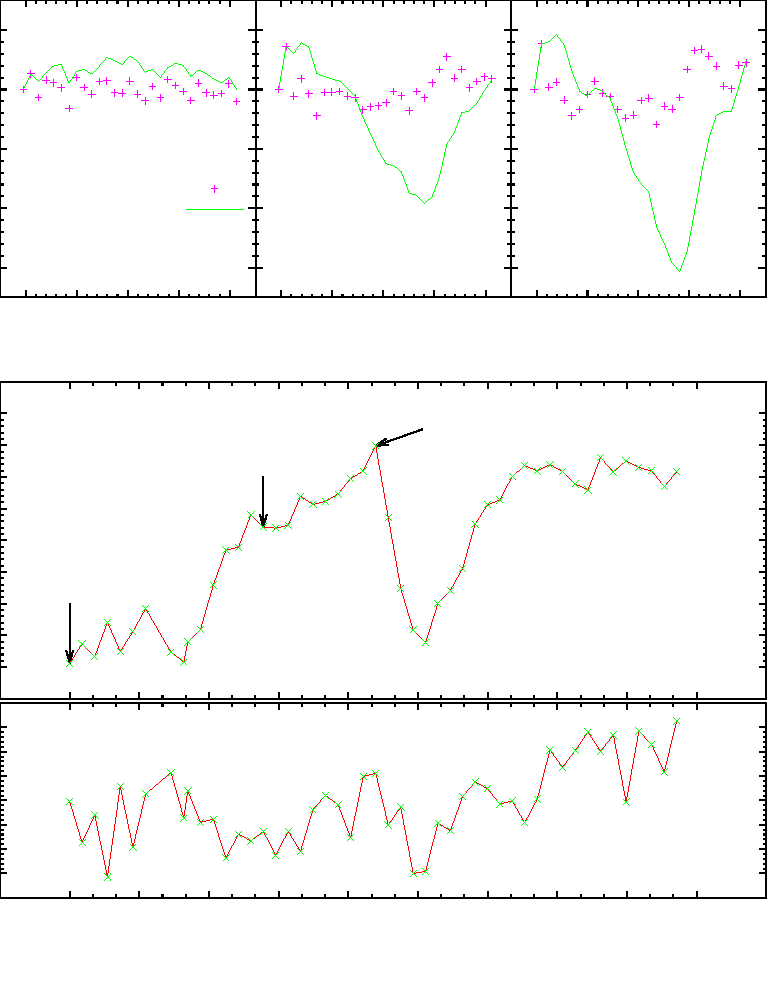
\includegraphics{linearitaet_verlauf}}%
    \gplfronttext
  \end{picture}%
\endgroup
